\section{Results – Strategy S3: Multi-LLM Consensus (Full)}
\label{sec:eval-s3}

The \textbf{S3: Multi-LLM Consensus (Full)} strategy runs multiple LLMs on the full document and aggregates their outputs with a verification/consensus step. We evaluate three variants: \textbf{S3.0} without few-shot examples on the original MUC-4 dataset, \textbf{S3.1} with few-shot examples on the original dataset, and \textbf{S3.2} with few-shot examples on a speech-style variant of MUC-4.

Figure~\ref{fig:s3-variants-bar} shows that adding both consensus and few-shot prompting (S3.1) strengthens the multi-model strategy by improving overall accuracy and reducing hallucinations compared to S3.0. The gains are concentrated in metrics that reflect correct and confident fills, indicating that cross-model agreement helps filter out unreliable predictions. The speech-style variant (S3.2) performs close to S3.1, suggesting that consensus mitigates much of the noise introduced by ASR-like phrasing. Compared to the single-pass baseline, S3.1 keeps overall accuracy similar but produces higher-quality nonempty predictions, reflecting the value of aggregating multiple model outputs.

\begin{figure}[H]
\centering
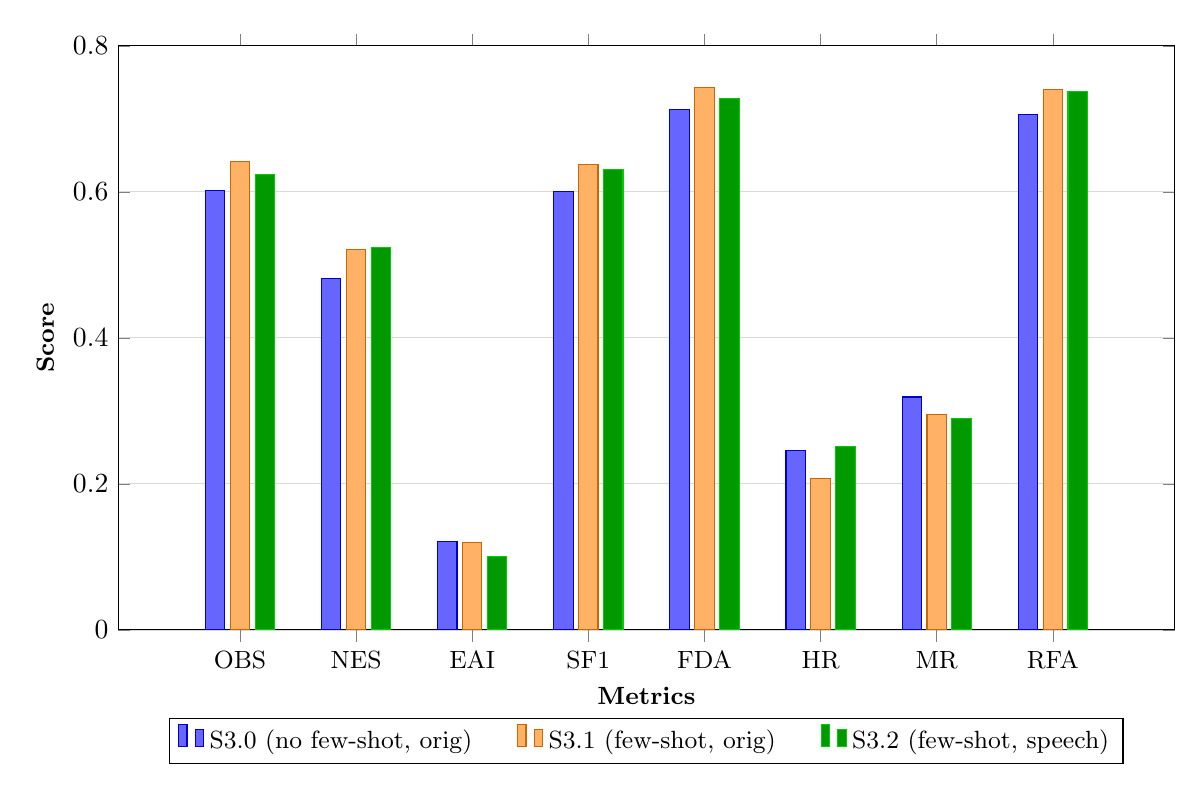
\begin{tikzpicture}
  \begin{axis}[
    width=15cm,
    height=9cm,
    ybar,
    bar width=7pt,
    ylabel={Score},
    ylabel style={font=\small\bfseries},
    xlabel={Metrics},
    xlabel style={font=\small\bfseries},
    symbolic x coords={OBS, NES, EAI, SF1, FDA, HR, MR, RFA},
    xtick=data,
    xticklabel style={font=\small},
    ymin=0,
    ymax=0.8,
    ytick={0, 0.2, 0.4, 0.6, 0.8},
    ymajorgrids=true,
    grid style={line width=0.3pt, draw=gray!30},
    legend style={
      at={(0.5,-0.15)},
      anchor=north,
      legend columns=3,
      font=\small,
      /tikz/every even column/.append style={column sep=0.5cm}
    },
    enlarge x limits=0.15,
  ]
  
  % S3.0 (no few-shot, orig) - Blue
  \addplot[fill=blue!60, draw=blue!80!black] coordinates {
    (OBS, 0.602)
    (NES, 0.481)
    (EAI, 0.121)
    (SF1, 0.601)
    (FDA, 0.713)
    (HR, 0.246)
    (MR, 0.319)
    (RFA, 0.706)
  };
  \addlegendentry{S3.0 (no few-shot, orig)}
  
  % S3.1 (few-shot, orig) - Orange
  \addplot[fill=orange!60, draw=orange!80!black] coordinates {
    (OBS, 0.641)
    (NES, 0.521)
    (EAI, 0.120)
    (SF1, 0.638)
    (FDA, 0.743)
    (HR, 0.208)
    (MR, 0.295)
    (RFA, 0.740)
  };
  \addlegendentry{S3.1 (few-shot, orig)}
  
  % S3.2 (few-shot, speech) - Green
  \addplot[fill=green!60!black, draw=green!80!black] coordinates {
    (OBS, 0.624)
    (NES, 0.524)
    (EAI, 0.100)
    (SF1, 0.630)
    (FDA, 0.728)
    (HR, 0.251)
    (MR, 0.289)
    (RFA, 0.738)
  };
  \addlegendentry{S3.2 (few-shot, speech)}
  
  \end{axis}
\end{tikzpicture}
\caption{Headline metrics for S3 variants on MUC-4 ($N{=}100$). 
The plot compares the multi-model consensus strategy across S3.0 (no few-shot), S3.1 
(few-shot), and S3.2 (few-shot with speech-style input). Few-shot prompting (S3.1) offers 
consistent gains in overall accuracy (OBS), schema adherence (FDA), and fully correct 
fields (RFA). The speech-style variant (S3.2) remains close to S3.1, showing that consensus 
aggregation reduces sensitivity to noise introduced by ASR-like phrasing.}
\label{fig:s3-variants-bar}
\end{figure}


\paragraph{Per-field behaviour (S3.1).}

Consensus is particularly strong for \texttt{perpetratorOrganization} and \texttt{weapon}; \texttt{perpetratorIndividual} remains hardest; \texttt{incidentLocation} improves compared to single-pass strategies.

Figure ~\ref{fig:s3-perfield-plot} illustrates how full-document consensus redistributes performance across individual slots. As in S1 and S2, \texttt{perpetratorOrganization} and \texttt{weapon} remain the easiest fields, with average scores of $0.756$ and $0.793$ respectively, reflecting that these categories are well supported by clear lexical cues and benefit from both models agreeing on salient mentions. \texttt{incidentStage} and \texttt{incidentDate} also perform strongly ($0.730$ for both), indicating that structured, temporally anchored information is well captured when the entire document is considered jointly. \texttt{incidentLocation} reaches $0.554$, which is higher than in the single-pass S1.1 setting and suggests that cross-model checking over the full context helps eliminate some location-related errors. In contrast, \texttt{perpetratorIndividual} remains comparatively weak ($0.561$), confirming that even an ensemble has difficulty with sparse and ambiguous references to individual actors. Overall, the field-level pattern supports the intuition that S3’s gains are concentrated in slots where multiple mentions and global cues are present, while inherently under-specified fields remain challenging.

\begin{figure}[H]
\centering
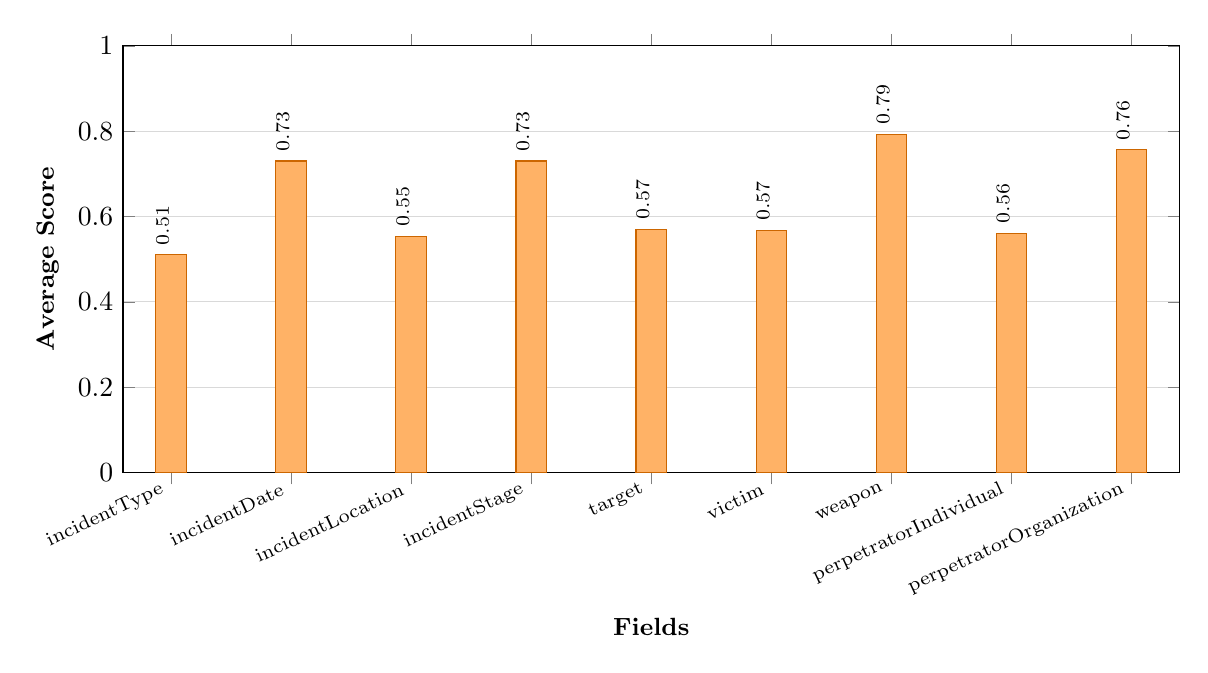
\begin{tikzpicture}
  \begin{axis}[
    width=15cm,
    height=7cm,
    ybar,
    bar width=11pt,
    ylabel={Average Score},
    ylabel style={font=\small\bfseries},
    xlabel={Fields},
    xlabel style={font=\small\bfseries},
    symbolic x coords={
      incidentType,
      incidentDate,
      incidentLocation,
      incidentStage,
      target,
      victim,
      weapon,
      perpetratorIndividual,
      perpetratorOrganization
    },
    xtick=data,
    xticklabel style={font=\scriptsize, rotate=25, anchor=east},
    ymin=0,
    ymax=1.0,
    ymajorgrids=true,
    grid style={line width=0.3pt, draw=gray!30},
    enlarge x limits=0.05,
    nodes near coords,
    nodes near coords style={
        font=\scriptsize,
        rotate=90,
        anchor=west,
        yshift=3pt
    }
  ]

  \addplot[fill=orange!60, draw=orange!80!black] coordinates {
    (incidentType, 0.510)
    (incidentDate, 0.730)
    (incidentLocation, 0.554)
    (incidentStage, 0.730)
    (target, 0.570)
    (victim, 0.567)
    (weapon, 0.793)
    (perpetratorIndividual, 0.561)
    (perpetratorOrganization, 0.756)
  };

  \end{axis}
\end{tikzpicture}

\caption{Per-field extraction performance for S3.1 on the MUC-4 subset ($N{=}100$). 
The consensus strategy improves stability across fields, with strong performance on 
structured attributes such as \textit{incidentDate}, \textit{incidentStage}, and 
\textit{weapon}. More open-ended fields like \textit{incidentType} and 
\textit{incidentLocation} remain comparatively difficult, reflecting the inherent 
ambiguity of these categories. Overall, S3.1 delivers a balanced improvement across 
most fields compared to non-consensus baselines.}
\label{fig:s3-perfield-plot}
\end{figure}



\subsection*{Latency}

Figure~\ref{fig:s3-latency-bar} highlights the computational cost of running multiple full-input models. S3.0 has a median latency of about $31$\,s per document and a moderate upper tail (p99 around $87$\,s). Incorporating few-shot examples in S3.1 increases the median latency to roughly $59$\,s and the mean to about $61$\,s, with a long tail that reaches $165$\,s, reflecting the overhead of larger prompts and dual model calls. S3.2, which operates on speech-style transcripts, is slightly faster than S3.1: its median and mean latencies drop to about $53$\,s and $55$\,s respectively, and the tail is somewhat shorter (p99 around $105$\,s). Compared to the single-pass few-shot strategy S1.1, S3.1 is slower in the median but has a somewhat shorter extreme tail (p99 $118.3$\,s vs.\ $134.9$\,s), suggesting that the cost of consensus is predictable but not catastrophic. In practice, S3 therefore occupies a middle ground in the accuracy–latency space: more expensive than S1 and S2, but still feasible for batched or asynchronous processing.

\begin{figure}[H]
\centering
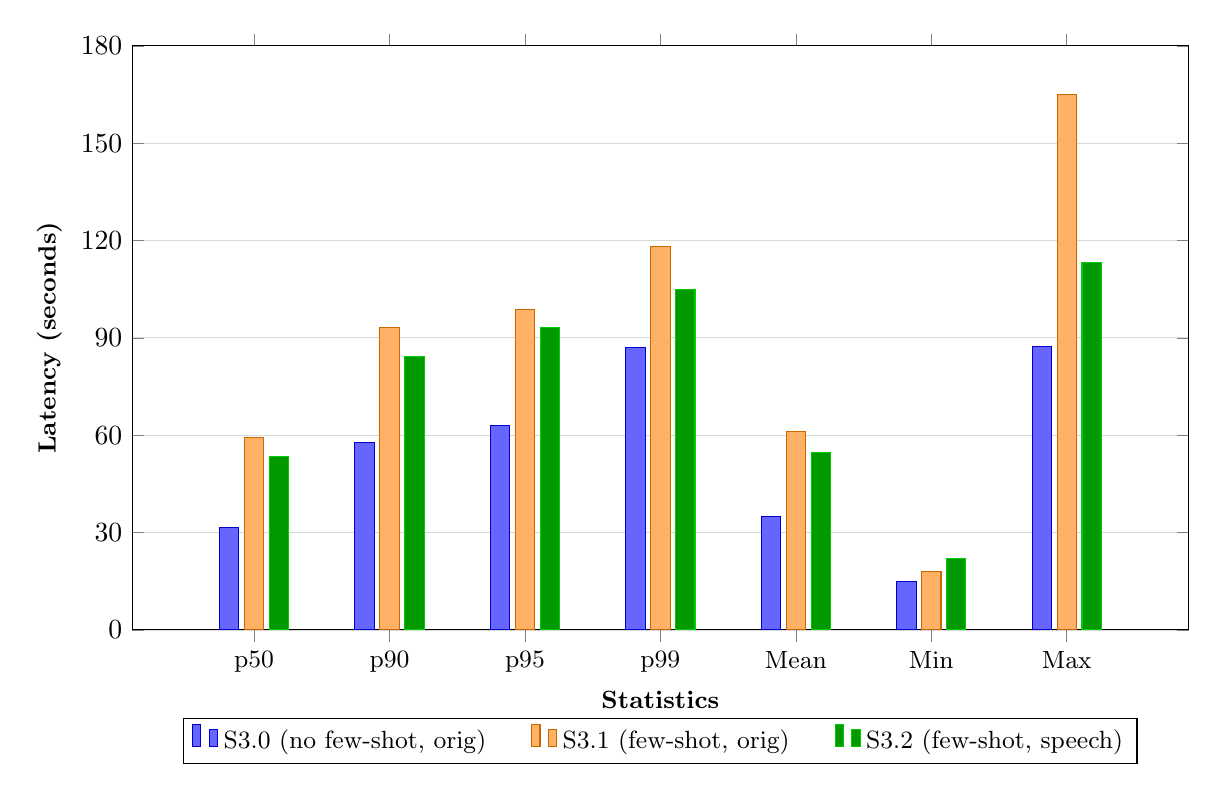
\begin{tikzpicture}
  \begin{axis}[
    width=15cm,
    height=9cm,
    ybar,
    bar width=7pt,
    ylabel={Latency (seconds)},
    ylabel style={font=\small\bfseries},
    xlabel={Statistics},
    xlabel style={font=\small\bfseries},
    symbolic x coords={p50, p90, p95, p99, Mean, Min, Max},
    xtick=data,
    xticklabel style={font=\small},
    ymin=0,
    ymax=180,
    ytick={0, 30, 60, 90, 120, 150, 180},
    ymajorgrids=true,
    grid style={line width=0.3pt, draw=gray!30},
    legend style={
      at={(0.5,-0.15)},
      anchor=north,
      legend columns=3,
      font=\small,
      /tikz/every even column/.append style={column sep=0.5cm}
    },
    enlarge x limits=0.15,
  ]
  
  % S3.0 (no few-shot, orig) - Blue
  \addplot[fill=blue!60, draw=blue!80!black] coordinates {
    (p50, 31.47)
    (p90, 57.79)
    (p95, 63.02)
    (p99, 87.16)
    (Mean, 34.83)
    (Min, 14.85)
    (Max, 87.24)
  };
  \addlegendentry{S3.0 (no few-shot, orig)}
  
  % S3.1 (few-shot, orig) - Orange
  \addplot[fill=orange!60, draw=orange!80!black] coordinates {
    (p50, 59.39)
    (p90, 93.15)
    (p95, 98.77)
    (p99, 118.28)
    (Mean, 61.09)
    (Min, 18.13)
    (Max, 164.96)
  };
  \addlegendentry{S3.1 (few-shot, orig)}
  
  % S3.2 (few-shot, speech) - Green
  \addplot[fill=green!60!black, draw=green!80!black] coordinates {
    (p50, 53.45)
    (p90, 84.15)
    (p95, 93.31)
    (p99, 104.99)
    (Mean, 54.55)
    (Min, 22.01)
    (Max, 113.26)
  };
  \addlegendentry{S3.2 (few-shot, speech)}
  
  \end{axis}
\end{tikzpicture}
\caption{Latency statistics for S3 variants (seconds). 
The multi-model consensus strategy exhibits substantially higher latency than single-model
approaches, with S3.1 (few-shot) producing the largest delays due to multiple model calls
combined with longer prompts. The speech-style configuration (S3.2) reduces extreme
latencies compared to S3.1 but remains significantly slower than the no–few-shot baseline
(S3.0). These results highlight the computational cost of consensus-based extraction, where
improved robustness and accuracy come at the expense of markedly increased processing time.}

\label{fig:s3-latency-bar}
\end{figure}


\subsection*{Cost Analysis (S3: Multi-LLM Consensus, Full Input)}

\textbf{Assumptions.} Two parallel extractions are run on the full input: one with \textit{GPT-5} and one with \textit{Gemini~2.5~Pro}, each using $I{=}3{,}000$ input tokens and $O{=}300$ output tokens. A single arbiter/verification step runs on \textit{GPT-5-mini} with $V_{\text{in}}{=}1{,}000$ and $V_{\text{out}}{=}100$. If audio is used, Whisper transcription for $D$ minutes is added once per record.

\textbf{Prices.} GPT-5: input \$1.25/M, output \$10.00/M; GPT-5-mini: input \$0.25/M, output \$2.00/M; Gemini~2.5~Pro (prompts $\le$200k): input \$1.25/M, output \$10.00/M; Whisper: \$0.006/min.

\textbf{Formula.}
\[
\text{Cost}_{\text{S3}} =
\Big(\tfrac{I}{10^6}p_{\text{in}}^{(5)}+\tfrac{O}{10^6}p_{\text{out}}^{(5)}\Big)
+\Big(\tfrac{I}{10^6}p_{\text{in}}^{(\text{Gemini})}+\tfrac{O}{10^6}p_{\text{out}}^{(\text{Gemini})}\Big)
+\Big(\tfrac{V_{\text{in}}}{10^6}p_{\text{in}}^{(\text{mini})}+\tfrac{V_{\text{out}}}{10^6}p_{\text{out}}^{(\text{mini})}\Big)
+0.006\cdot D
\]

\textbf{Per-record (no audio).}
\[
\begin{aligned}
\text{GPT-5 extract: } & \tfrac{3000}{10^6}\!\cdot\!1.25 + \tfrac{300}{10^6}\!\cdot\!10.00 = \mathbf{\$0.00675} \\
\text{Gemini~2.5~Pro extract: } & \tfrac{3000}{10^6}\!\cdot\!1.25 + \tfrac{300}{10^6}\!\cdot\!10.00 = \mathbf{\$0.00675} \\
\text{mini arbiter: } & \tfrac{1000}{10^6}\!\cdot\!0.25 + \tfrac{100}{10^6}\!\cdot\!2.00 = \mathbf{\$0.00045} \\
\textbf{Total: } & \mathbf{\$0.01395}\ (\approx 1.40\text{¢/doc})
\end{aligned}
\]

\textbf{With audio (Whisper).} Adding Whisper introduces a linear term $0.006\cdot D$. For $D{=}1$\,min, the total cost becomes $\$0.01395 + 0.006 = \mathbf{\$0.01995}$ (approximately $2.00$\,¢ per document). Under these settings, S3 costs roughly $1.9\times$ as much as S1 (\$0.01395 vs.\ \$0.00720 per document, no audio), reflecting the dual full-input passes while keeping the arbiter overhead small compared to the extraction steps.

\subsection*{Consistency (Formatting \& Style)}

\begin{figure}[H]
\centering
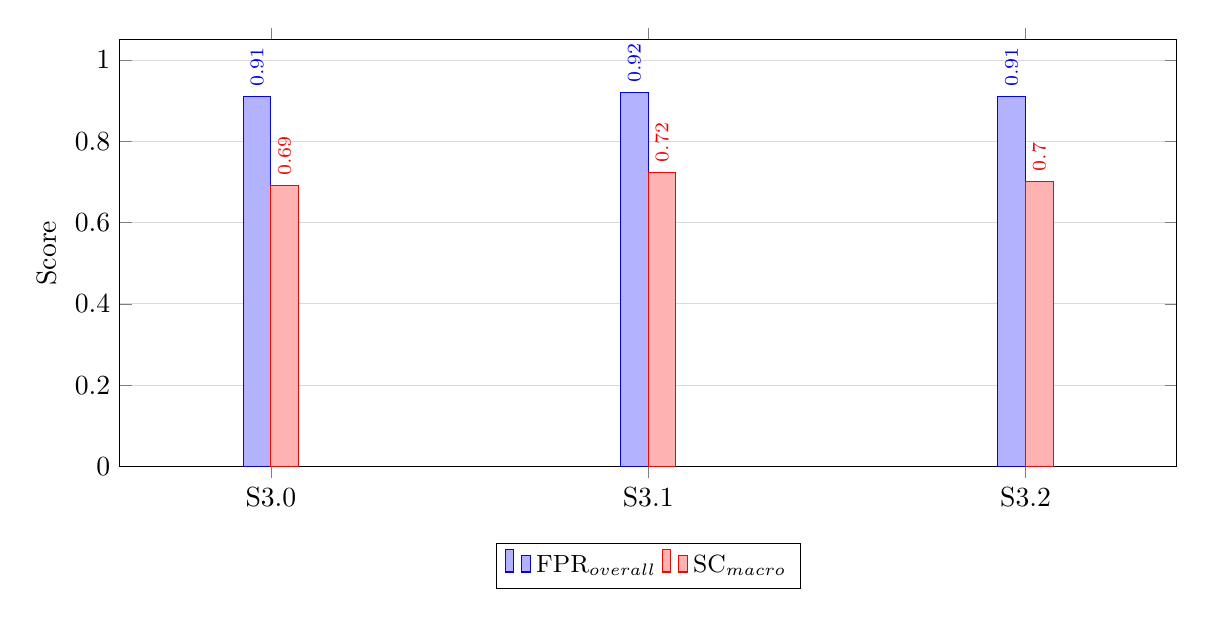
\begin{tikzpicture}
  \begin{axis}[
    width=15cm,
    height=7cm,
    ybar=0pt,
    bar width=10pt,
    ymin=0, ymax=1.05,
    ylabel={Score},
    symbolic x coords={S3.0,S3.1,S3.2},
    xtick=data,
    ymajorgrids=true,
    grid style={line width=0.3pt, draw=gray!30},
    legend style={at={(0.5,-0.18)}, anchor=north, legend columns=2, font=\small},
    enlarge x limits=0.20,
    nodes near coords,
    nodes near coords style={
        font=\scriptsize,
        rotate=90,     % vertical text
        anchor=west,
    }
  ]

    % FPR_overall
    \addplot coordinates {(S3.0,0.910) (S3.1,0.920) (S3.2,0.910)};
    \addlegendentry{$\mathrm{FPR}_{\text{overall}}$}

    % SC_macro
    \addplot coordinates {(S3.0,0.691) (S3.1,0.724) (S3.2,0.702)};
    \addlegendentry{$\mathrm{SC}_{\text{macro}}$}
  \end{axis}
\end{tikzpicture}
\caption{Consistency (S3 variants): schema formatting vs.\ input-aware style.}
\label{fig:s3-consistency}
\end{figure}

Figure~\ref{fig:s3-consistency} indicates that multi-LLM consensus maintains high structural and stylistic consistency. All S3 variants achieve $\mathrm{FPR}_{\text{overall}}{=}0.910$ or higher, with S3.1 slightly ahead at $0.920$, which shows that most outputs adhere to the expected JSON schema even after aggregation. The style-aware score $\mathrm{SC}_{\text{macro}}$ improves from $0.691$ in S3.0 to $0.724$ in S3.1, suggesting that the combination of few-shot prompting and consensus helps the system converge on more uniform phrasing and formatting across documents. S3.2, evaluated on speech-style input, remains close to S3.1 in both metrics, which indicates that the ensemble design is robust to noisier transcripts: consensus can smooth out some of the variability introduced by speech-like text while preserving schema fidelity.

Taken together, the S3 family demonstrates how full-document multi-LLM consensus trades additional cost and latency for improved calibration and robustness. Relative to the iterative S2.1 configuration, S3.1 reduces hallucinations (HR $0.301 \rightarrow 0.208$) and raises FDA (from $0.718$ to $0.743$) while also achieving higher OBS, suggesting that cross-model agreement provides more trustworthy fills at the expense of a small increase in misses. Compared to the best single-pass configuration S1.1, S3.1 reaches very similar headline scores but offers better performance on gold-nonempty slots (higher NES) and slightly lower MR, indicating stronger content quality when fields are present. The speech-style variant S3.2 maintains this pattern, trading a small decrease in overall accuracy for higher NES and stable RFA, which makes it attractive for spoken-text deployments where correctness on filled slots is more important than exploiting empty–empty alignment. Overall, S3 is best suited for settings where accuracy, calibration, and robustness justify a roughly twofold increase in LLM cost over S1 and a moderate latency premium.
